\documentclass[]{article}
\usepackage{lmodern}
\usepackage{amssymb,amsmath}
\usepackage{ifxetex,ifluatex}
\usepackage{fixltx2e} % provides \textsubscript
\ifnum 0\ifxetex 1\fi\ifluatex 1\fi=0 % if pdftex
  \usepackage[T1]{fontenc}
  \usepackage[utf8]{inputenc}
\else % if luatex or xelatex
  \ifxetex
    \usepackage{mathspec}
  \else
    \usepackage{fontspec}
  \fi
  \defaultfontfeatures{Ligatures=TeX,Scale=MatchLowercase}
\fi
% use upquote if available, for straight quotes in verbatim environments
\IfFileExists{upquote.sty}{\usepackage{upquote}}{}
% use microtype if available
\IfFileExists{microtype.sty}{%
\usepackage{microtype}
\UseMicrotypeSet[protrusion]{basicmath} % disable protrusion for tt fonts
}{}
\usepackage{hyperref}
\hypersetup{unicode=true,
            pdftitle={purr::map() demo for Code review},
            pdfauthor={PennCHOP microbiome program, Scott Garrett Daniel},
            pdfborder={0 0 0},
            breaklinks=true}
\urlstyle{same}  % don't use monospace font for urls
\usepackage{color}
\usepackage{fancyvrb}
\newcommand{\VerbBar}{|}
\newcommand{\VERB}{\Verb[commandchars=\\\{\}]}
\DefineVerbatimEnvironment{Highlighting}{Verbatim}{commandchars=\\\{\}}
% Add ',fontsize=\small' for more characters per line
\usepackage{framed}
\definecolor{shadecolor}{RGB}{248,248,248}
\newenvironment{Shaded}{\begin{snugshade}}{\end{snugshade}}
\newcommand{\KeywordTok}[1]{\textcolor[rgb]{0.13,0.29,0.53}{\textbf{#1}}}
\newcommand{\DataTypeTok}[1]{\textcolor[rgb]{0.13,0.29,0.53}{#1}}
\newcommand{\DecValTok}[1]{\textcolor[rgb]{0.00,0.00,0.81}{#1}}
\newcommand{\BaseNTok}[1]{\textcolor[rgb]{0.00,0.00,0.81}{#1}}
\newcommand{\FloatTok}[1]{\textcolor[rgb]{0.00,0.00,0.81}{#1}}
\newcommand{\ConstantTok}[1]{\textcolor[rgb]{0.00,0.00,0.00}{#1}}
\newcommand{\CharTok}[1]{\textcolor[rgb]{0.31,0.60,0.02}{#1}}
\newcommand{\SpecialCharTok}[1]{\textcolor[rgb]{0.00,0.00,0.00}{#1}}
\newcommand{\StringTok}[1]{\textcolor[rgb]{0.31,0.60,0.02}{#1}}
\newcommand{\VerbatimStringTok}[1]{\textcolor[rgb]{0.31,0.60,0.02}{#1}}
\newcommand{\SpecialStringTok}[1]{\textcolor[rgb]{0.31,0.60,0.02}{#1}}
\newcommand{\ImportTok}[1]{#1}
\newcommand{\CommentTok}[1]{\textcolor[rgb]{0.56,0.35,0.01}{\textit{#1}}}
\newcommand{\DocumentationTok}[1]{\textcolor[rgb]{0.56,0.35,0.01}{\textbf{\textit{#1}}}}
\newcommand{\AnnotationTok}[1]{\textcolor[rgb]{0.56,0.35,0.01}{\textbf{\textit{#1}}}}
\newcommand{\CommentVarTok}[1]{\textcolor[rgb]{0.56,0.35,0.01}{\textbf{\textit{#1}}}}
\newcommand{\OtherTok}[1]{\textcolor[rgb]{0.56,0.35,0.01}{#1}}
\newcommand{\FunctionTok}[1]{\textcolor[rgb]{0.00,0.00,0.00}{#1}}
\newcommand{\VariableTok}[1]{\textcolor[rgb]{0.00,0.00,0.00}{#1}}
\newcommand{\ControlFlowTok}[1]{\textcolor[rgb]{0.13,0.29,0.53}{\textbf{#1}}}
\newcommand{\OperatorTok}[1]{\textcolor[rgb]{0.81,0.36,0.00}{\textbf{#1}}}
\newcommand{\BuiltInTok}[1]{#1}
\newcommand{\ExtensionTok}[1]{#1}
\newcommand{\PreprocessorTok}[1]{\textcolor[rgb]{0.56,0.35,0.01}{\textit{#1}}}
\newcommand{\AttributeTok}[1]{\textcolor[rgb]{0.77,0.63,0.00}{#1}}
\newcommand{\RegionMarkerTok}[1]{#1}
\newcommand{\InformationTok}[1]{\textcolor[rgb]{0.56,0.35,0.01}{\textbf{\textit{#1}}}}
\newcommand{\WarningTok}[1]{\textcolor[rgb]{0.56,0.35,0.01}{\textbf{\textit{#1}}}}
\newcommand{\AlertTok}[1]{\textcolor[rgb]{0.94,0.16,0.16}{#1}}
\newcommand{\ErrorTok}[1]{\textcolor[rgb]{0.64,0.00,0.00}{\textbf{#1}}}
\newcommand{\NormalTok}[1]{#1}
\usepackage{graphicx,grffile}
\makeatletter
\def\maxwidth{\ifdim\Gin@nat@width>\linewidth\linewidth\else\Gin@nat@width\fi}
\def\maxheight{\ifdim\Gin@nat@height>\textheight\textheight\else\Gin@nat@height\fi}
\makeatother
% Scale images if necessary, so that they will not overflow the page
% margins by default, and it is still possible to overwrite the defaults
% using explicit options in \includegraphics[width, height, ...]{}
\setkeys{Gin}{width=\maxwidth,height=\maxheight,keepaspectratio}
\IfFileExists{parskip.sty}{%
\usepackage{parskip}
}{% else
\setlength{\parindent}{0pt}
\setlength{\parskip}{6pt plus 2pt minus 1pt}
}
\setlength{\emergencystretch}{3em}  % prevent overfull lines
\providecommand{\tightlist}{%
  \setlength{\itemsep}{0pt}\setlength{\parskip}{0pt}}
\setcounter{secnumdepth}{0}
% Redefines (sub)paragraphs to behave more like sections
\ifx\paragraph\undefined\else
\let\oldparagraph\paragraph
\renewcommand{\paragraph}[1]{\oldparagraph{#1}\mbox{}}
\fi
\ifx\subparagraph\undefined\else
\let\oldsubparagraph\subparagraph
\renewcommand{\subparagraph}[1]{\oldsubparagraph{#1}\mbox{}}
\fi

%%% Use protect on footnotes to avoid problems with footnotes in titles
\let\rmarkdownfootnote\footnote%
\def\footnote{\protect\rmarkdownfootnote}


  \title{purr::map() demo for Code review}
    \author{PennCHOP microbiome program, Scott Garrett Daniel}
      \date{\today}

\usepackage{pdflscape}
\usepackage{lscape}
\usepackage{tikz}
\usepackage{tikz-cd}
\usepackage{color}
\usepackage[colorinlistoftodos]{todonotes}

\newcommand{\blandscape}{\begin{landscape}}
\newcommand{\elandscape}{\end{landscape}}

\newcommand{\bscript}{\begin{scriptsize}}
\newcommand{\escript}{\end{scriptsize}}

\newcommand{\stopdocument}{\end{document}} % \newcommand cannot define that starts with \end... so use \stopdocument instead of \enddocument

\def\red{\textcolor{red}}
\def\green{\textcolor{green}}
\def\blue{\textcolor{blue}}

\begin{document}
\maketitle

{
\setcounter{tocdepth}{3}
}

\includegraphics{logo_blk.png}\\
\tableofcontents

\section{Packages and setting up
data}\label{packages-and-setting-up-data}

Based on:
\url{https://aosmith.rbind.io/2019/07/22/automate-model-fitting-with-loops/}

\begin{Shaded}
\begin{Highlighting}[]
\CommentTok{#devtools::install_github("thomasp85/patchwork")}
\KeywordTok{library}\NormalTok{(purrr) }\CommentTok{# v. 0.3.2}
\KeywordTok{library}\NormalTok{(ggplot2) }\CommentTok{# v. 3.2.0}
\KeywordTok{library}\NormalTok{(patchwork) }\CommentTok{# v. 0.0.1, github only, see above ^}
\KeywordTok{library}\NormalTok{(broom) }\CommentTok{# v. 0.5.2}

\NormalTok{dat =}\StringTok{ }\KeywordTok{structure}\NormalTok{(}\KeywordTok{list}\NormalTok{(}\DataTypeTok{group =} \KeywordTok{structure}\NormalTok{(}\KeywordTok{c}\NormalTok{(1L, 1L, 1L, 1L, 1L, 1L, 1L, }
\NormalTok{1L, 1L, 1L, 1L, 1L, 1L, 1L, 1L, 2L, 2L, 2L, 2L, 2L, 2L, 2L, 2L, }
\NormalTok{2L, 2L, 2L, 2L, 2L, 2L, 2L), }\DataTypeTok{.Label =} \KeywordTok{c}\NormalTok{(}\StringTok{"a"}\NormalTok{, }\StringTok{"b"}\NormalTok{), }\DataTypeTok{class =} \StringTok{"factor"}\NormalTok{), }
    \DataTypeTok{resp =} \KeywordTok{c}\NormalTok{(}\FloatTok{10.48}\NormalTok{, }\FloatTok{9.87}\NormalTok{, }\FloatTok{11.1}\NormalTok{, }\FloatTok{8.56}\NormalTok{, }\FloatTok{11.15}\NormalTok{, }\FloatTok{9.53}\NormalTok{, }\FloatTok{8.99}\NormalTok{, }\FloatTok{10.06}\NormalTok{, }
    \FloatTok{11.02}\NormalTok{, }\FloatTok{10.57}\NormalTok{, }\FloatTok{11.85}\NormalTok{, }\FloatTok{10.11}\NormalTok{, }\FloatTok{9.25}\NormalTok{, }\FloatTok{11.66}\NormalTok{, }\FloatTok{10.72}\NormalTok{, }\FloatTok{8.34}\NormalTok{, }\FloatTok{10.58}\NormalTok{, }
    \FloatTok{10.47}\NormalTok{, }\FloatTok{9.46}\NormalTok{, }\FloatTok{11.13}\NormalTok{, }\FloatTok{8.35}\NormalTok{, }\FloatTok{9.69}\NormalTok{, }\FloatTok{9.82}\NormalTok{, }\FloatTok{11.47}\NormalTok{, }\FloatTok{9.13}\NormalTok{, }\FloatTok{11.53}\NormalTok{, }
    \FloatTok{11.05}\NormalTok{, }\FloatTok{11.03}\NormalTok{, }\FloatTok{10.84}\NormalTok{, }\FloatTok{10.22}\NormalTok{), }\DataTypeTok{slp =} \KeywordTok{c}\NormalTok{(}\FloatTok{38.27}\NormalTok{, }\FloatTok{46.33}\NormalTok{, }\FloatTok{44.29}\NormalTok{, }
    \FloatTok{35.57}\NormalTok{, }\FloatTok{34.78}\NormalTok{, }\FloatTok{47.81}\NormalTok{, }\FloatTok{50.45}\NormalTok{, }\FloatTok{46.31}\NormalTok{, }\FloatTok{47.82}\NormalTok{, }\FloatTok{42.07}\NormalTok{, }\FloatTok{31.75}\NormalTok{, }\FloatTok{65.65}\NormalTok{, }
    \FloatTok{47.42}\NormalTok{, }\FloatTok{41.51}\NormalTok{, }\FloatTok{38.69}\NormalTok{, }\FloatTok{47.84}\NormalTok{, }\FloatTok{46.22}\NormalTok{, }\FloatTok{50.66}\NormalTok{, }\FloatTok{50.69}\NormalTok{, }\FloatTok{44.09}\NormalTok{, }\FloatTok{47.3}\NormalTok{, }
    \FloatTok{52.53}\NormalTok{, }\FloatTok{53.63}\NormalTok{, }\FloatTok{53.38}\NormalTok{, }\FloatTok{27.34}\NormalTok{, }\FloatTok{51.83}\NormalTok{, }\FloatTok{56.63}\NormalTok{, }\FloatTok{32.99}\NormalTok{, }\FloatTok{77.5}\NormalTok{, }\FloatTok{38.24}
\NormalTok{    ), }\DataTypeTok{grad =} \KeywordTok{c}\NormalTok{(}\FloatTok{0.3}\NormalTok{, }\FloatTok{0.66}\NormalTok{, }\FloatTok{0.57}\NormalTok{, }\FloatTok{0.23}\NormalTok{, }\FloatTok{0.31}\NormalTok{, }\FloatTok{0.48}\NormalTok{, }\FloatTok{0.5}\NormalTok{, }\FloatTok{0.49}\NormalTok{, }
    \FloatTok{2.41}\NormalTok{, }\FloatTok{0.6}\NormalTok{, }\FloatTok{0.27}\NormalTok{, }\FloatTok{0.89}\NormalTok{, }\FloatTok{2.43}\NormalTok{, }\FloatTok{1.02}\NormalTok{, }\FloatTok{2.17}\NormalTok{, }\FloatTok{1.38}\NormalTok{, }\FloatTok{0.17}\NormalTok{, }\FloatTok{0.47}\NormalTok{, }
    \FloatTok{1.1}\NormalTok{, }\FloatTok{3.28}\NormalTok{, }\FloatTok{6.14}\NormalTok{, }\FloatTok{3.8}\NormalTok{, }\FloatTok{4.35}\NormalTok{, }\FloatTok{0.85}\NormalTok{, }\FloatTok{1.13}\NormalTok{, }\FloatTok{1.11}\NormalTok{, }\FloatTok{2.93}\NormalTok{, }\FloatTok{1.13}\NormalTok{, }
    \FloatTok{4.52}\NormalTok{, }\FloatTok{0.13}\NormalTok{)), }\DataTypeTok{class =} \StringTok{"data.frame"}\NormalTok{, }\DataTypeTok{row.names =} \KeywordTok{c}\NormalTok{(}\OtherTok{NA}\NormalTok{, }\OperatorTok{-}\NormalTok{30L) )}
\KeywordTok{head}\NormalTok{(dat)}
\end{Highlighting}
\end{Shaded}

\begin{verbatim}
##   group  resp   slp grad
## 1     a 10.48 38.27 0.30
## 2     a  9.87 46.33 0.66
## 3     a 11.10 44.29 0.57
## 4     a  8.56 35.57 0.23
## 5     a 11.15 34.78 0.31
## 6     a  9.53 47.81 0.48
\end{verbatim}

\section{Function for model
generation}\label{function-for-model-generation}

\begin{Shaded}
\begin{Highlighting}[]
\NormalTok{ttest_fun =}\StringTok{ }\ControlFlowTok{function}\NormalTok{(response) \{}
\NormalTok{  form =}\StringTok{ }\KeywordTok{paste}\NormalTok{(response, }\StringTok{"~ group"}\NormalTok{)}
  \KeywordTok{lm}\NormalTok{(}\KeywordTok{as.formula}\NormalTok{(form), }\DataTypeTok{data =}\NormalTok{ dat)}
\NormalTok{\}}
\KeywordTok{ttest_fun}\NormalTok{(}\DataTypeTok{response =} \StringTok{"resp"}\NormalTok{)}
\end{Highlighting}
\end{Shaded}

\begin{verbatim}
## 
## Call:
## lm(formula = as.formula(form), data = dat)
## 
## Coefficients:
## (Intercept)       groupb  
##     10.3280      -0.1207
\end{verbatim}

\section{Set names for vars we want to
model}\label{set-names-for-vars-we-want-to-model}

\begin{Shaded}
\begin{Highlighting}[]
\NormalTok{vars =}\StringTok{ }\KeywordTok{names}\NormalTok{(dat)[}\DecValTok{2}\OperatorTok{:}\DecValTok{4}\NormalTok{]}
\NormalTok{vars}
\end{Highlighting}
\end{Shaded}

\begin{verbatim}
## [1] "resp" "slp"  "grad"
\end{verbatim}

\begin{Shaded}
\begin{Highlighting}[]
\NormalTok{vars =}\StringTok{ }\KeywordTok{set_names}\NormalTok{(vars)}
\NormalTok{vars}
\end{Highlighting}
\end{Shaded}

\begin{verbatim}
##   resp    slp   grad 
## "resp"  "slp" "grad"
\end{verbatim}

\section{Map the model to each var}\label{map-the-model-to-each-var}

\begin{Shaded}
\begin{Highlighting}[]
\NormalTok{models =}\StringTok{ }\NormalTok{vars }\OperatorTok
\StringTok{     }\KeywordTok{map}\NormalTok{(ttest_fun)}
\NormalTok{models}
\end{Highlighting}
\end{Shaded}

\begin{verbatim}
## $resp
## 
## Call:
## lm(formula = as.formula(form), data = dat)
## 
## Coefficients:
## (Intercept)       groupb  
##     10.3280      -0.1207  
## 
## 
## $slp
## 
## Call:
## lm(formula = as.formula(form), data = dat)
## 
## Coefficients:
## (Intercept)       groupb  
##       43.91         4.81  
## 
## 
## $grad
## 
## Call:
## lm(formula = as.formula(form), data = dat)
## 
## Coefficients:
## (Intercept)       groupb  
##      0.8887       1.2773
\end{verbatim}

\begin{Shaded}
\begin{Highlighting}[]
\CommentTok{#same thing rather than set_names in above code block}
\CommentTok{# vars %>%}
\CommentTok{#      set_names() %>%}
\CommentTok{#      map(ttest_fun)}
\end{Highlighting}
\end{Shaded}

\section{Create a ggplot graph
function}\label{create-a-ggplot-graph-function}

\begin{Shaded}
\begin{Highlighting}[]
\NormalTok{resid_plots =}\StringTok{ }\ControlFlowTok{function}\NormalTok{(model, modelname) \{}
\NormalTok{     output =}\StringTok{ }\KeywordTok{augment}\NormalTok{(model) }\CommentTok{#extract residuals and fitted values via broom::augment()}
     
\NormalTok{     res.v.fit =}\StringTok{ }\KeywordTok{ggplot}\NormalTok{(output, }\KeywordTok{aes}\NormalTok{(}\DataTypeTok{x =}\NormalTok{ .fitted, }\DataTypeTok{y =}\NormalTok{ .resid) ) }\OperatorTok{+}
\StringTok{          }\KeywordTok{geom_point}\NormalTok{() }\OperatorTok{+}
\StringTok{          }\KeywordTok{theme_bw}\NormalTok{(}\DataTypeTok{base_size =} \DecValTok{16}\NormalTok{)}
     
\NormalTok{     res.box =}\StringTok{ }\KeywordTok{ggplot}\NormalTok{(output, }\KeywordTok{aes}\NormalTok{(}\DataTypeTok{x =} \StringTok{""}\NormalTok{, }\DataTypeTok{y =}\NormalTok{ .resid) ) }\OperatorTok{+}
\StringTok{          }\KeywordTok{geom_boxplot}\NormalTok{() }\OperatorTok{+}
\StringTok{          }\KeywordTok{theme_bw}\NormalTok{(}\DataTypeTok{base_size =} \DecValTok{16}\NormalTok{) }\OperatorTok{+}
\StringTok{          }\KeywordTok{labs}\NormalTok{(}\DataTypeTok{x =} \OtherTok{NULL}\NormalTok{)}
     
\NormalTok{     res.v.fit }\OperatorTok{+}\StringTok{ }\NormalTok{res.box }\OperatorTok{+}
\StringTok{          }\KeywordTok{plot_annotation}\NormalTok{(}\DataTypeTok{title =} \KeywordTok{paste}\NormalTok{(}\StringTok{"Residuals plots for"}\NormalTok{, modelname) ) }
\CommentTok{# plot_annotation is part of patchwork and glues together the individual plots}
\NormalTok{\}}
\end{Highlighting}
\end{Shaded}

\section{Loop through models and graph each
one}\label{loop-through-models-and-graph-each-one}

\begin{Shaded}
\begin{Highlighting}[]
\CommentTok{#for one model:}
\CommentTok{#resid_plots(model = models[[1]], modelname = names(models)[1])}

\CommentTok{#loop through all models}
\NormalTok{residplots =}\StringTok{ }\KeywordTok{imap}\NormalTok{(models, resid_plots)}
\NormalTok{residplots}
\end{Highlighting}
\end{Shaded}

\begin{verbatim}
## $resp
\end{verbatim}

\begin{center}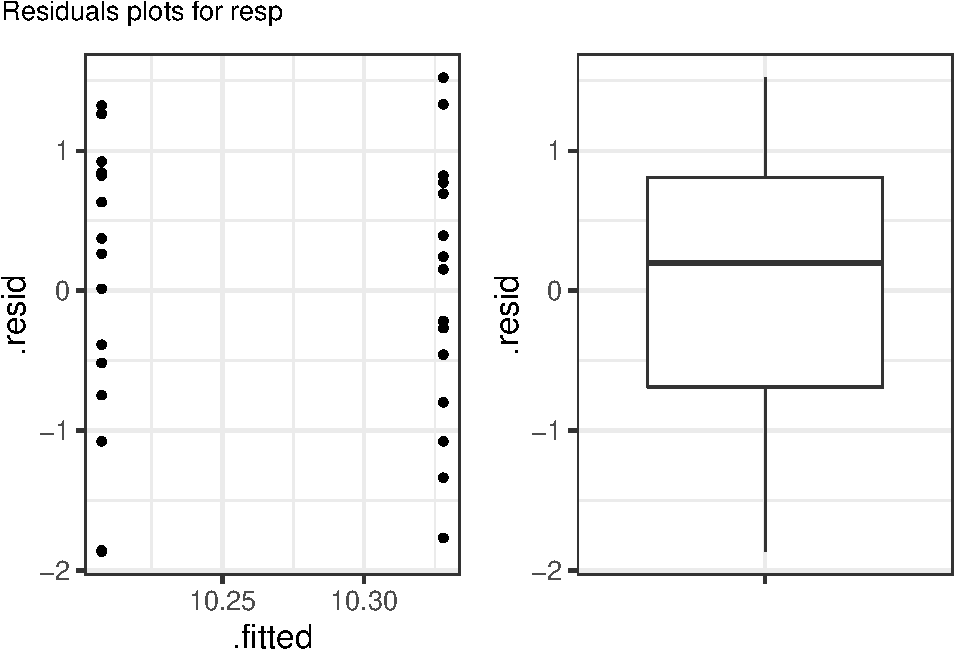
\includegraphics{purr_map_demo_files/figure-latex/unnamed-chunk-6-1} \end{center}

\begin{verbatim}
## 
## $slp
\end{verbatim}

\begin{center}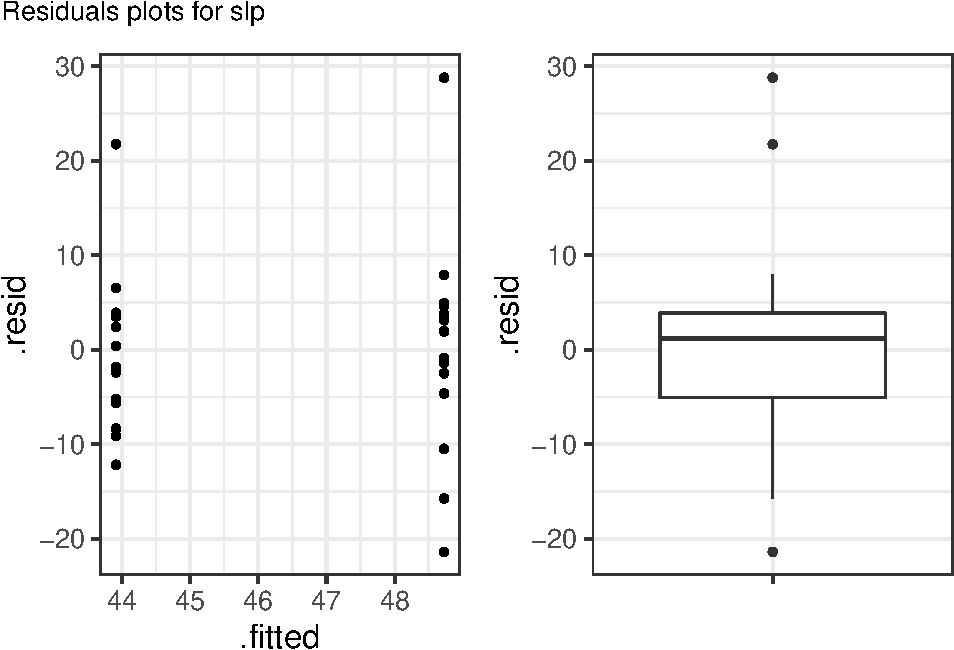
\includegraphics{purr_map_demo_files/figure-latex/unnamed-chunk-6-2} \end{center}

\begin{verbatim}
## 
## $grad
\end{verbatim}

\begin{center}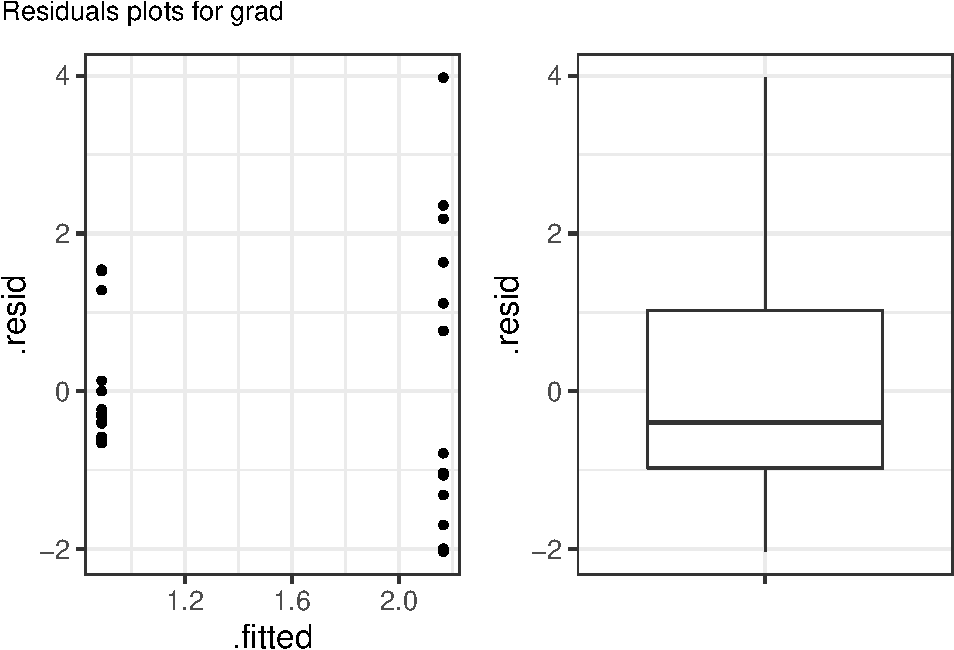
\includegraphics{purr_map_demo_files/figure-latex/unnamed-chunk-6-3} \end{center}

\section{Updating one of the models or
subsetting}\label{updating-one-of-the-models-or-subsetting}

\begin{Shaded}
\begin{Highlighting}[]
\NormalTok{gradmod =}\StringTok{ }\KeywordTok{ttest_fun}\NormalTok{(}\StringTok{"log(grad)"}\NormalTok{)}

\NormalTok{models}\OperatorTok{$}\NormalTok{log_grad =}\StringTok{ }\NormalTok{gradmod}
\NormalTok{models}\OperatorTok{$}\NormalTok{grad =}\StringTok{ }\OtherTok{NULL}
\NormalTok{models}
\end{Highlighting}
\end{Shaded}

\begin{verbatim}
## $resp
## 
## Call:
## lm(formula = as.formula(form), data = dat)
## 
## Coefficients:
## (Intercept)       groupb  
##     10.3280      -0.1207  
## 
## 
## $slp
## 
## Call:
## lm(formula = as.formula(form), data = dat)
## 
## Coefficients:
## (Intercept)       groupb  
##       43.91         4.81  
## 
## 
## $log_grad
## 
## Call:
## lm(formula = as.formula(form), data = dat)
## 
## Coefficients:
## (Intercept)       groupb  
##     -0.4225       0.7177
\end{verbatim}

\begin{Shaded}
\begin{Highlighting}[]
\NormalTok{models[}\OperatorTok{!}\KeywordTok{names}\NormalTok{(models) }\OperatorTok\StringTok{ "slp"}\NormalTok{]}
\end{Highlighting}
\end{Shaded}

\begin{verbatim}
## $resp
## 
## Call:
## lm(formula = as.formula(form), data = dat)
## 
## Coefficients:
## (Intercept)       groupb  
##     10.3280      -0.1207  
## 
## 
## $log_grad
## 
## Call:
## lm(formula = as.formula(form), data = dat)
## 
## Coefficients:
## (Intercept)       groupb  
##     -0.4225       0.7177
\end{verbatim}

\section{Extracting statistics from the
models}\label{extracting-statistics-from-the-models}

\begin{Shaded}
\begin{Highlighting}[]
\NormalTok{res_anova =}\StringTok{ }\KeywordTok{map_dfr}\NormalTok{(models, tidy, }\DataTypeTok{conf.int =} \OtherTok{TRUE}\NormalTok{, }\DataTypeTok{.id =} \StringTok{"variable"}\NormalTok{) }

\CommentTok{#map_dfr and map_dfc return data frames by row-binding and col-binding respectively}
\NormalTok{res_anova}
\end{Highlighting}
\end{Shaded}

\begin{verbatim}
## # A tibble: 6 x 8
##   variable term    estimate std.error statistic  p.value conf.low conf.high
##   <chr>    <chr>      <dbl>     <dbl>     <dbl>    <dbl>    <dbl>     <dbl>
## 1 resp     (Inter~   10.3       0.260    39.7   3.60e-26   9.80     10.9   
## 2 resp     groupb    -0.121     0.368    -0.328 7.45e- 1  -0.874     0.632 
## 3 slp      (Inter~   43.9       2.56     17.2   2.18e-16  38.7      49.2   
## 4 slp      groupb     4.81      3.62      1.33  1.95e- 1  -2.61     12.2   
## 5 log_grad (Inter~   -0.423     0.255    -1.66  1.09e- 1  -0.945     0.0997
## 6 log_grad groupb     0.718     0.361     1.99  5.64e- 2  -0.0208    1.46
\end{verbatim}

\section{Example from one of the projects I'm working
on}\label{example-from-one-of-the-projects-im-working-on}

\subsection{Sample data}\label{sample-data}

\subsection{Important response and predictor
variables}\label{important-response-and-predictor-variables}

\begin{Shaded}
\begin{Highlighting}[]
\CommentTok{#in 16S bacterial data, we care about how the diversity changes from one condition to the next}
\NormalTok{responses =}\StringTok{ }\KeywordTok{c}\NormalTok{(}\StringTok{"shannon"}\NormalTok{, }\StringTok{"richness"}\NormalTok{, }\StringTok{"faith_pd"}\NormalTok{)}
\NormalTok{predictors =}\StringTok{ }\KeywordTok{c}\NormalTok{(}\StringTok{"Location"}\NormalTok{, }\StringTok{"study_day"}\NormalTok{)}
\end{Highlighting}
\end{Shaded}

\subsection{Modify ttest function}\label{modify-ttest-function}

\begin{Shaded}
\begin{Highlighting}[]
\NormalTok{ttest_funs =}\StringTok{ }\ControlFlowTok{function}\NormalTok{(response, predictor) \{}
  
\NormalTok{  form =}\StringTok{ }\KeywordTok{paste0}\NormalTok{(response, }\StringTok{" ~ "}\NormalTok{, predictor)}
  \KeywordTok{lm}\NormalTok{(}\KeywordTok{as.formula}\NormalTok{(form), }\DataTypeTok{data =}\NormalTok{ s)}
  
\NormalTok{\}}
\end{Highlighting}
\end{Shaded}

\subsection{Run it!}\label{run-it}

\begin{Shaded}
\begin{Highlighting}[]
\NormalTok{predictors =}\StringTok{ }\KeywordTok{set_names}\NormalTok{(predictors,predictors)}
\NormalTok{responses =}\StringTok{ }\KeywordTok{set_names}\NormalTok{(responses,responses)}

\ControlFlowTok{for}\NormalTok{ (x }\ControlFlowTok{in}\NormalTok{ predictors) \{}
\NormalTok{  responses }\OperatorTok
\StringTok{    }\KeywordTok{map}\NormalTok{(}\OperatorTok{~}\StringTok{ }\KeywordTok{ttest_funs}\NormalTok{(.,x))}
\NormalTok{\}}

\CommentTok{#map2(responses, predictors, ~ ttest_funs(.x,.y))}

\CommentTok{#ttest_fun(..1, ..2)}
\end{Highlighting}
\end{Shaded}


\end{document}
